\documentclass[]{article}

%opening

\usepackage{amsmath}
\usepackage{amsfonts}
\usepackage{float}
\usepackage{hyperref}
\usepackage[explicit]{titlesec}
\usepackage{xcolor}
\usepackage{graphicx}
\usepackage{indentfirst}

\title{B\&W Colorising Models\\Project Report 3\\Team MMM}
\author{
	Ashera Dyussenova\\
	\texttt{a.dyusenova@innopolis.university}
	\and
	Mark Zakharov\\
	\texttt{ma.zakharov@innopolis.university}
	\and
	Nikolay Pavlenko\\
	\texttt{n.pavlenko@innopolis.university}
}
\begin{document}
	\maketitle
	\section{Current Direction of the Work}
	The past few weeks we have decided on focus on better tailoring the hand-written CNN model for the colorization task by increasing the size of the training dataset to 5000 images (as much as memory on our limited computational resources allowed). We have also implemented the suggestion to predict HSL format rather than RGB in order to reduce the brownish effect on the colored photos, and experimented with different hyperparameters of the CNN.
	\\
	\section{HSL format}
	HSL (Hue, Saturation, Lightness), as opposed to RGB (Red, Green, Blue) are two different color models used in digital imaging, each offering distinct advantages. While RGB works by combining various intensities of red, green, and blue light to produce a broad spectrum of colors, HSL is a cylindrical-coordinate representation of colors, where Hue refers to the type of color (e.g., red, blue, green), Saturation defines the purity or vividness of the color, and Lightness determines the brightness from black to full intensity. \\
	
	In the context of image colorization task at hand, a colorization to HSL could offer more intuitive control over color adjustment due to its characteristics. HSL separates the representation of colors into components that are more relatable to human perception compared to the direct combinations of red, green, and blue channels in RGB. For colorization, HSL's separation of color (Hue), purity (Saturation), and lightness provides a significantly more natural way to manipulate and control the hues and saturation of colors in an image. It allows easier adjustments to the vividness and brightness without impacting the underlying color relationships, making it particularly useful in tasks like color grading or recoloring images where preserving the natural look and feel is crucial. The decoupling of intensity (lightness) from the pure color properties (hue and saturation) also could also be advantageous in image colorization by a deep neural network.
	\\
	\section{Changing Hyperparameters}
	
	In order to test the new colorization to HSL we have created three CNN models that share the same architecture as was used the previous week, but have different hyperparameters: 
	\begin{enumerate}
		\item \textbf{model1} has the same hyperparameters as the model that was employed in image colorization the previous week
		\item \textbf{model2} has stride of 2, rather than 1, to check how much of an influence it has on the accuracy of colorization
		\item \textbf{model3} has stride of 1, but it has a greater number of filters than model1, possibly allowing it to catch more rare and unique image features.
	\end{enumerate}
	
	\section{Colorization Results:}
	
	\begin{figure}[H]
		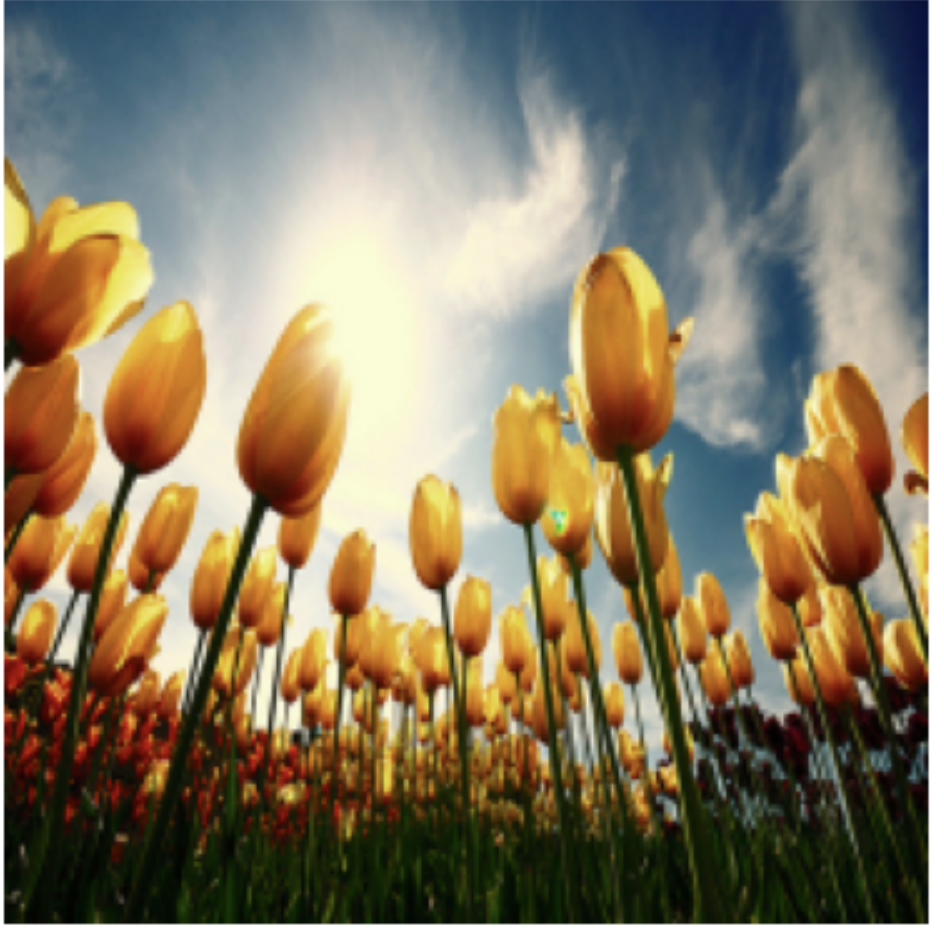
\includegraphics[scale=0.35]{orig_1.png}
		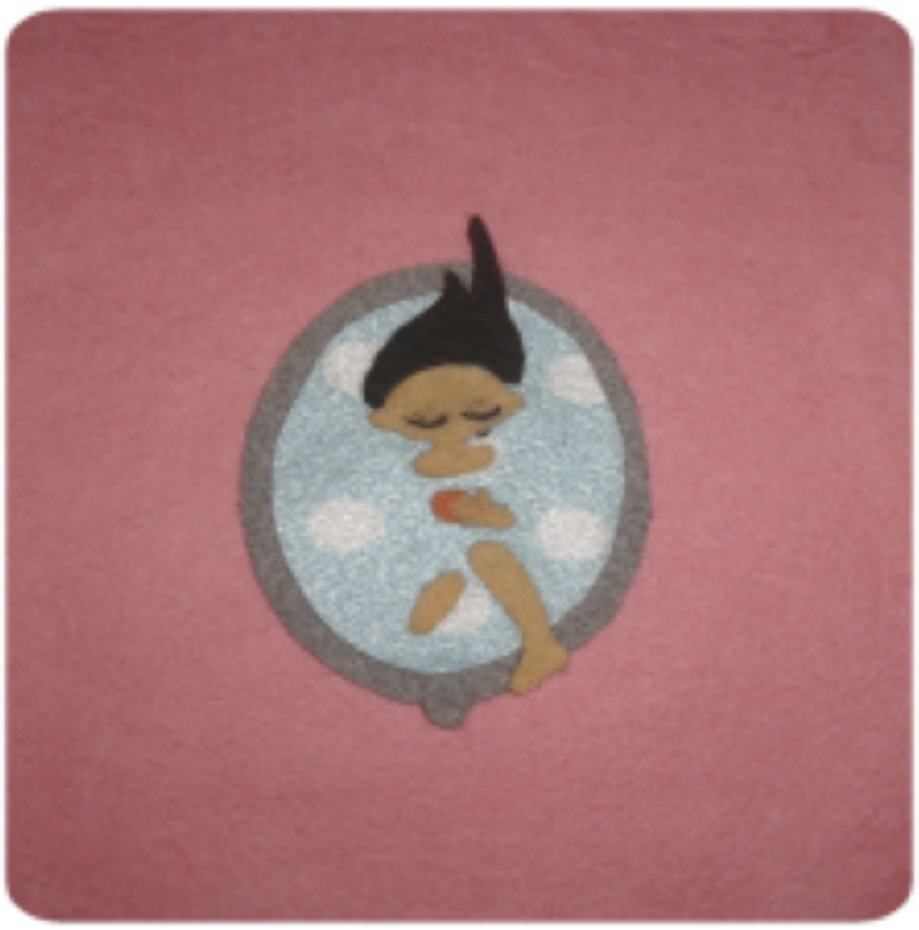
\includegraphics[scale=0.35]{orig_2.png}
		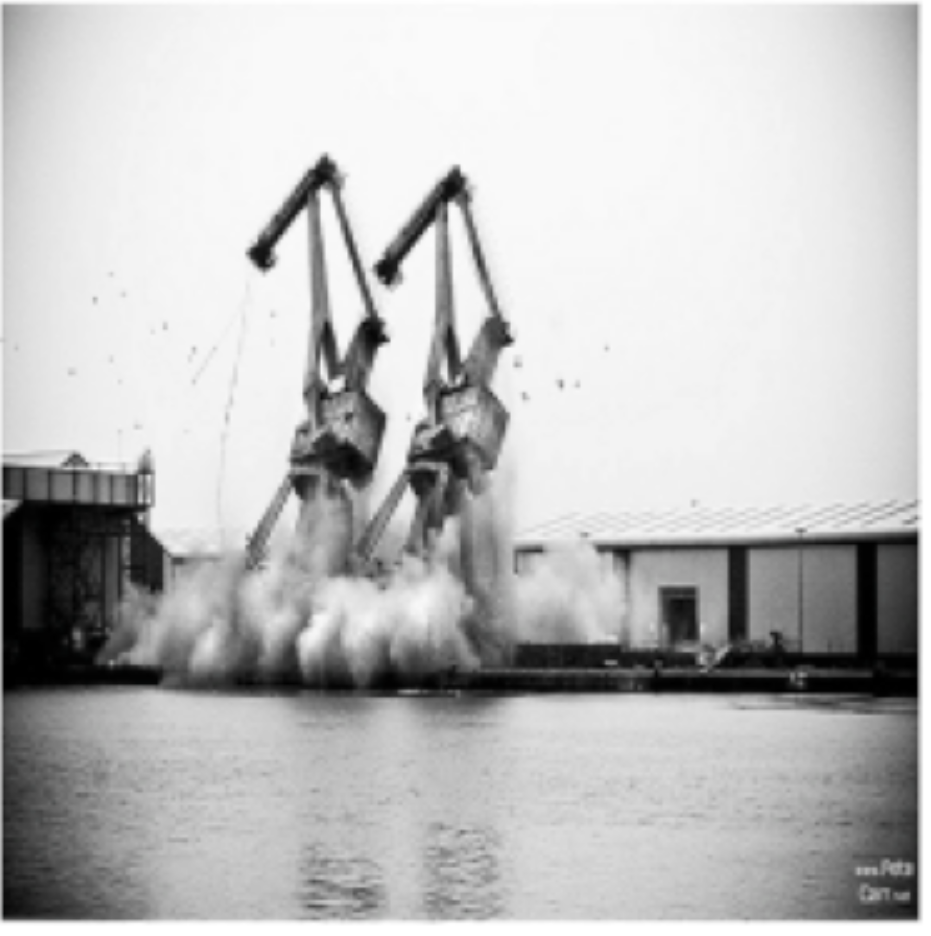
\includegraphics[scale=0.35]{orig_3.png}
		\caption{Original pictures/RGB colorizations}
	\end{figure}
	
	\begin{figure}[H]
		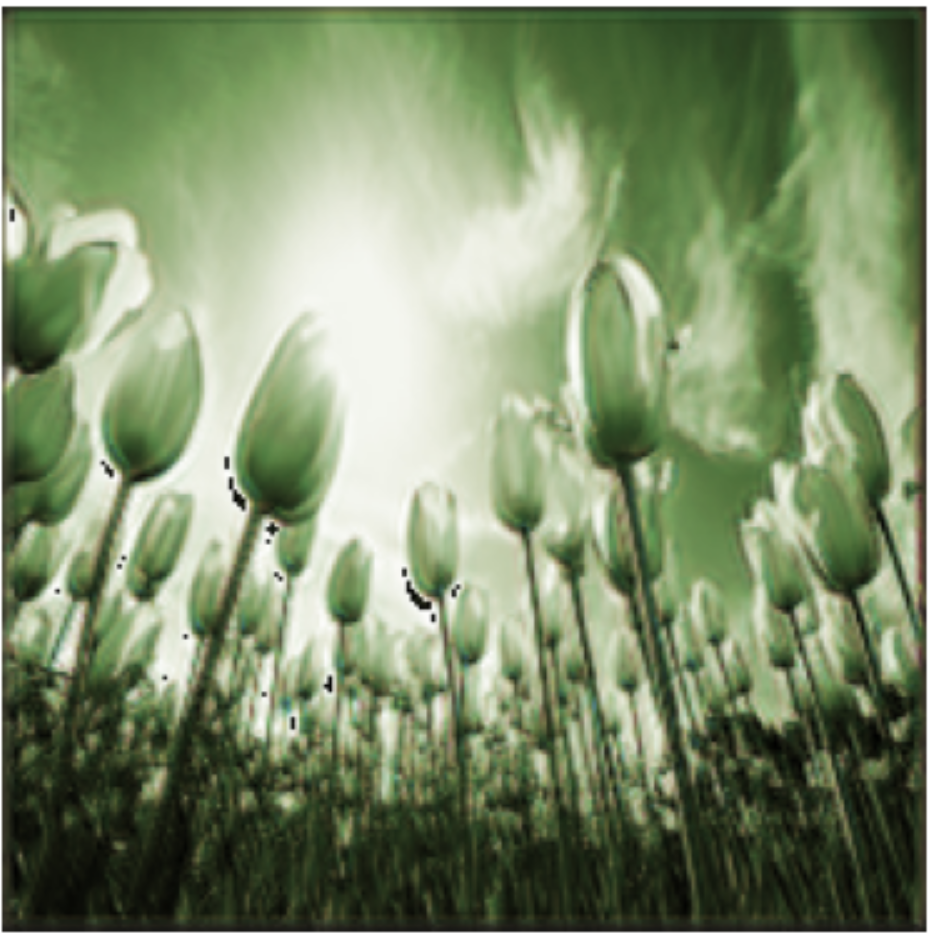
\includegraphics[scale=0.35]{m1_1.png}
		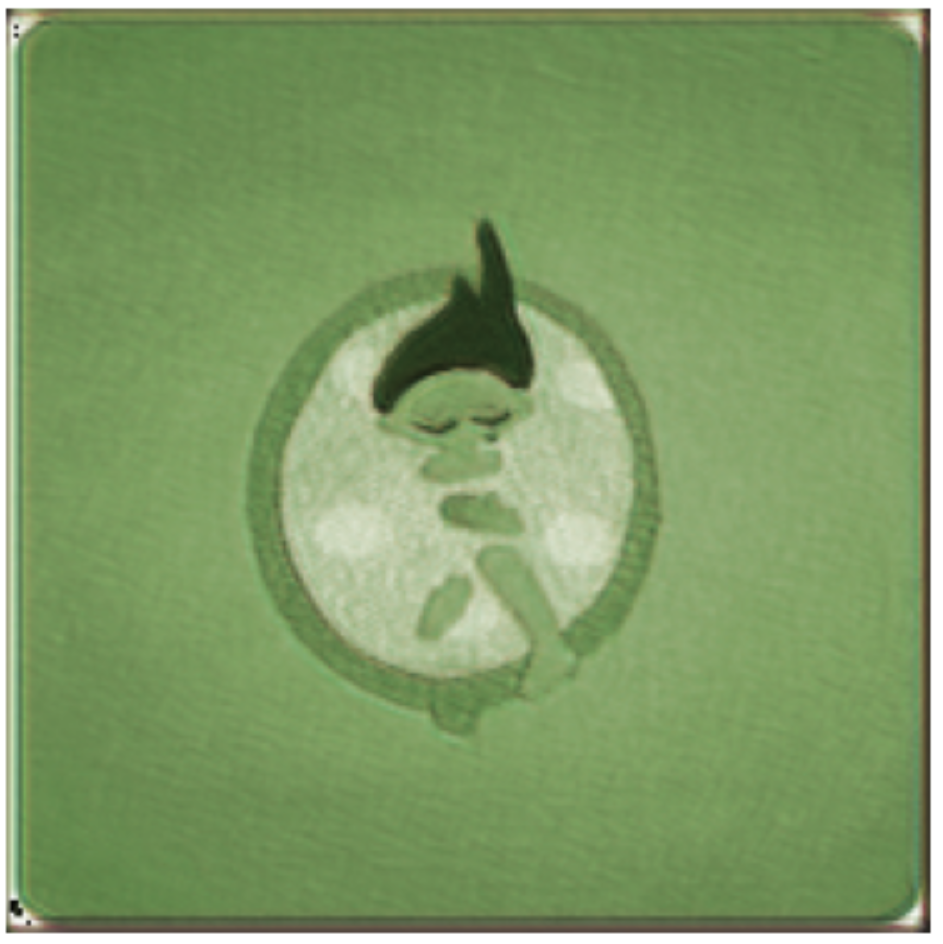
\includegraphics[scale=0.35]{m1_2.png}
		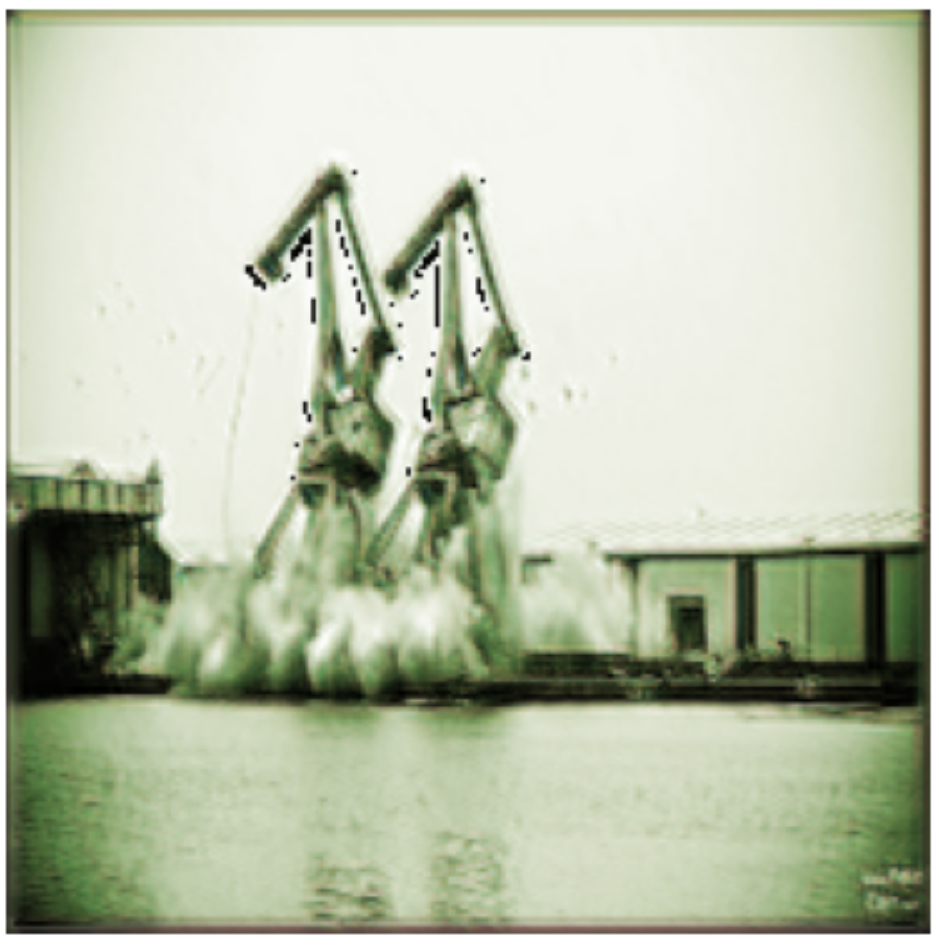
\includegraphics[scale=0.35]{m1_3.png}
		\caption{model1 colorizations}
	\end{figure}
	
	\begin{figure}[H]
		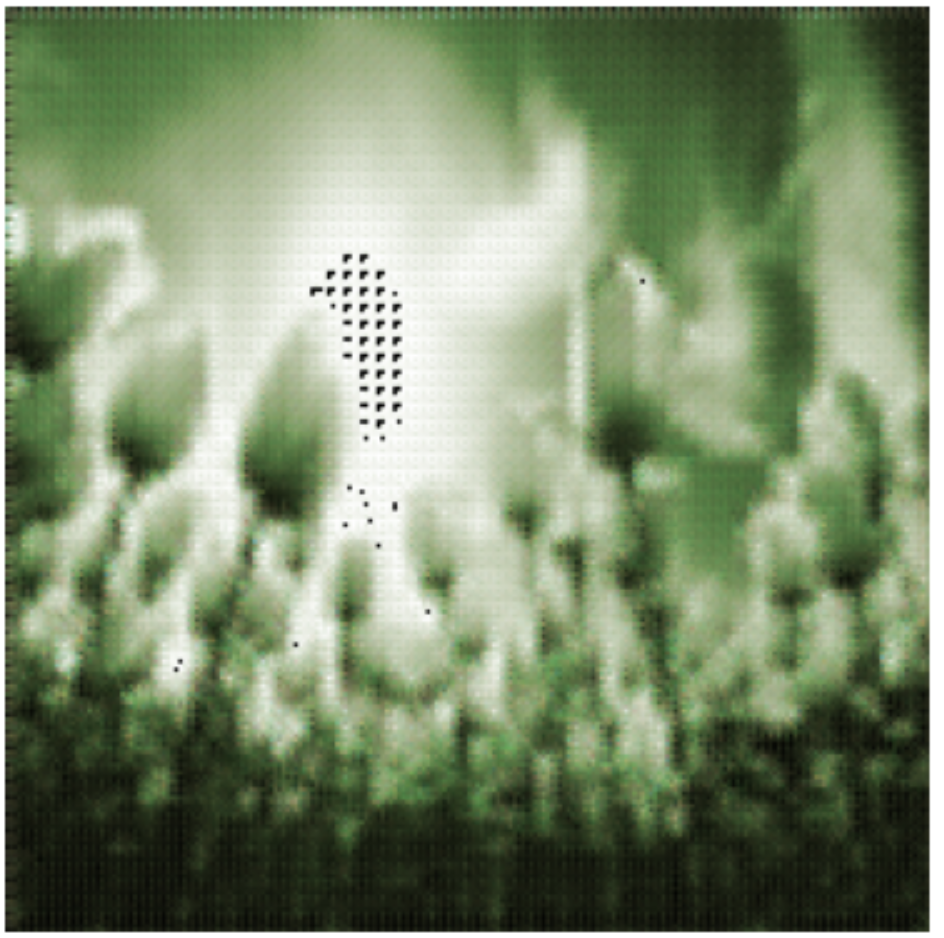
\includegraphics[scale=0.35]{m2_1.png}
		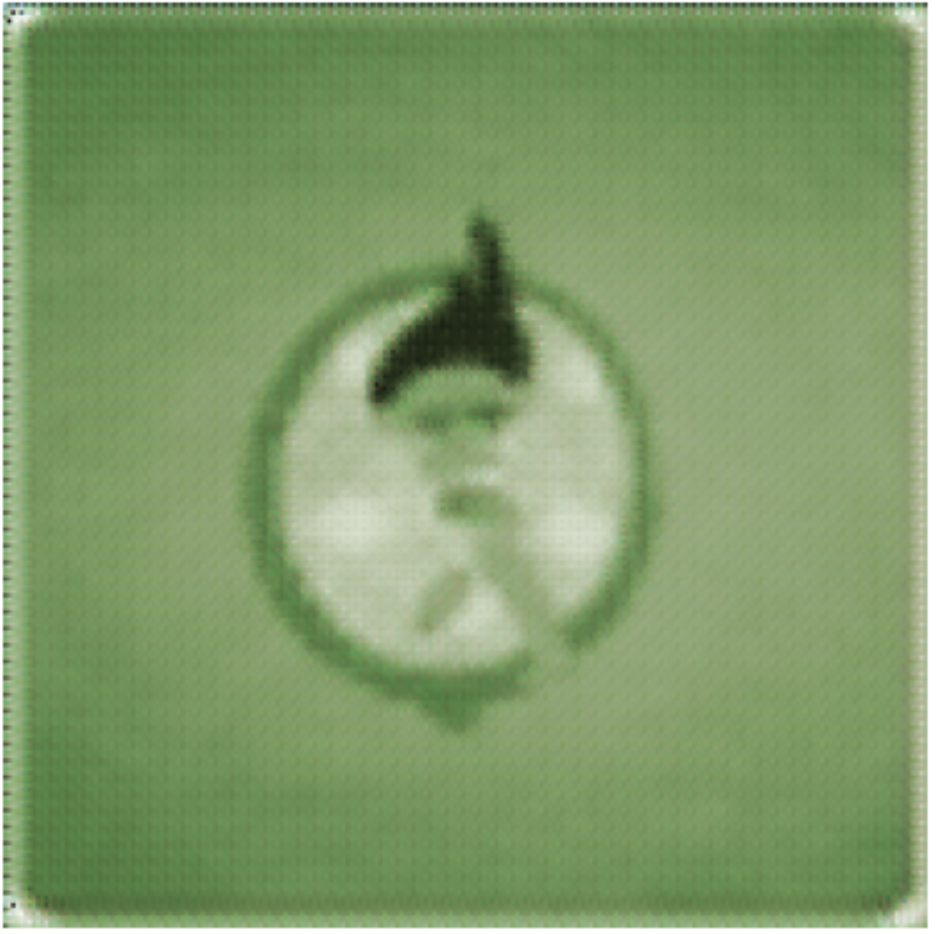
\includegraphics[scale=0.35]{m2_2.png}
		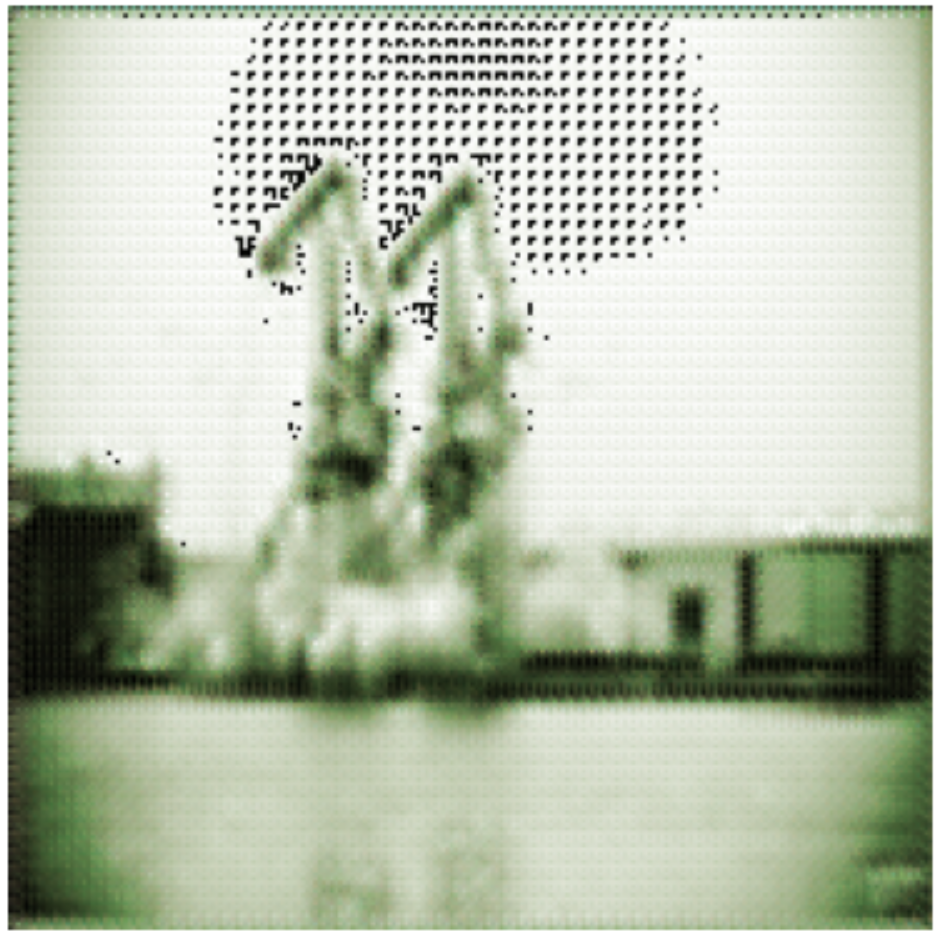
\includegraphics[scale=0.35]{m2_3.png}
		\caption{model2 colorizations}
	\end{figure}
	
	\begin{figure}[H]
		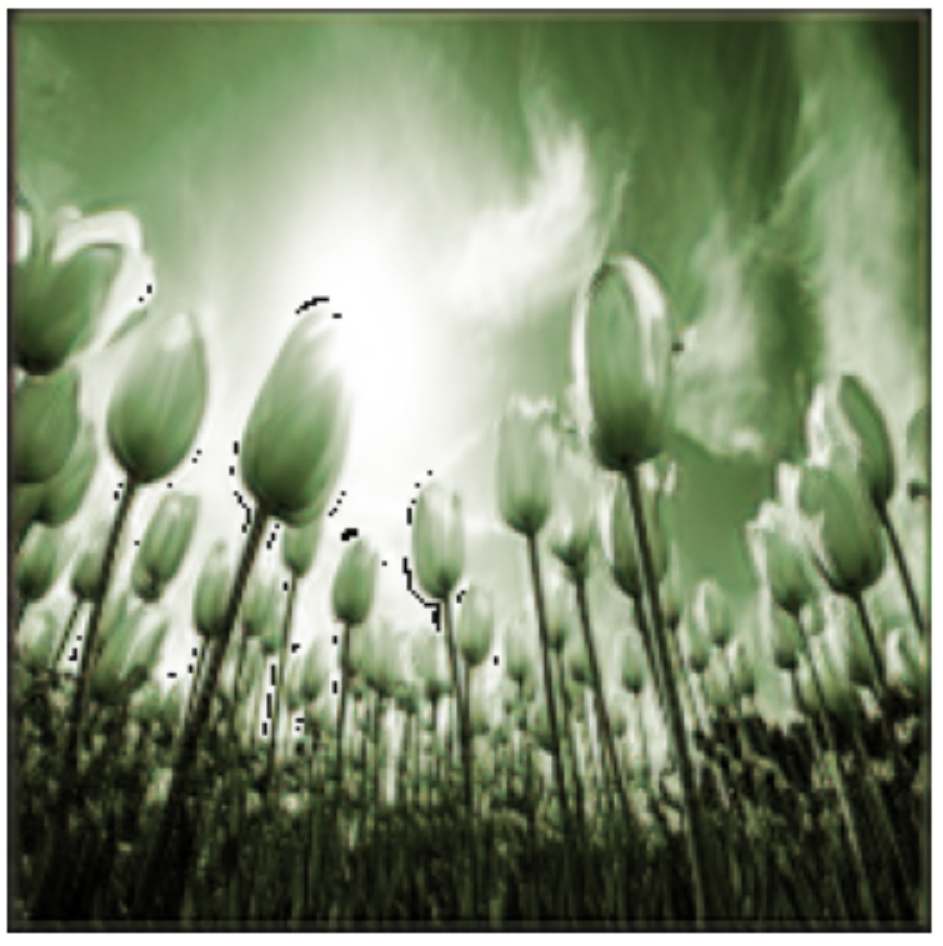
\includegraphics[scale=0.35]{m3_1.png}
		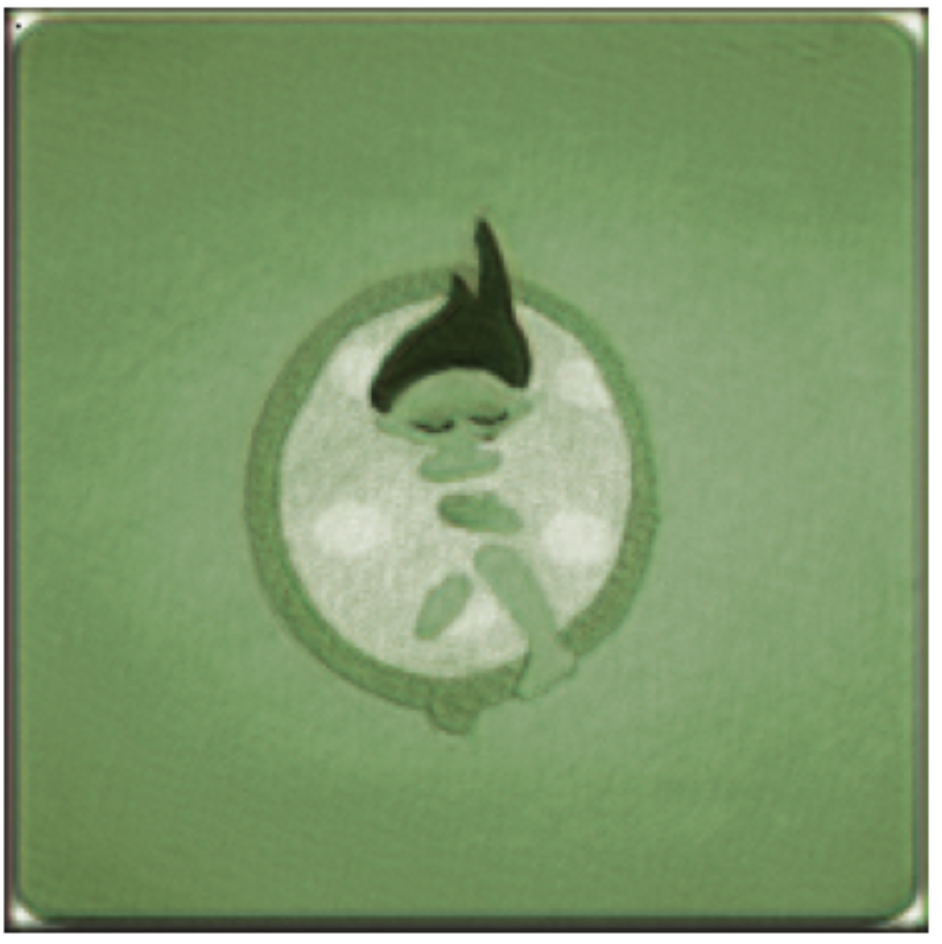
\includegraphics[scale=0.35]{m3_2.png}
		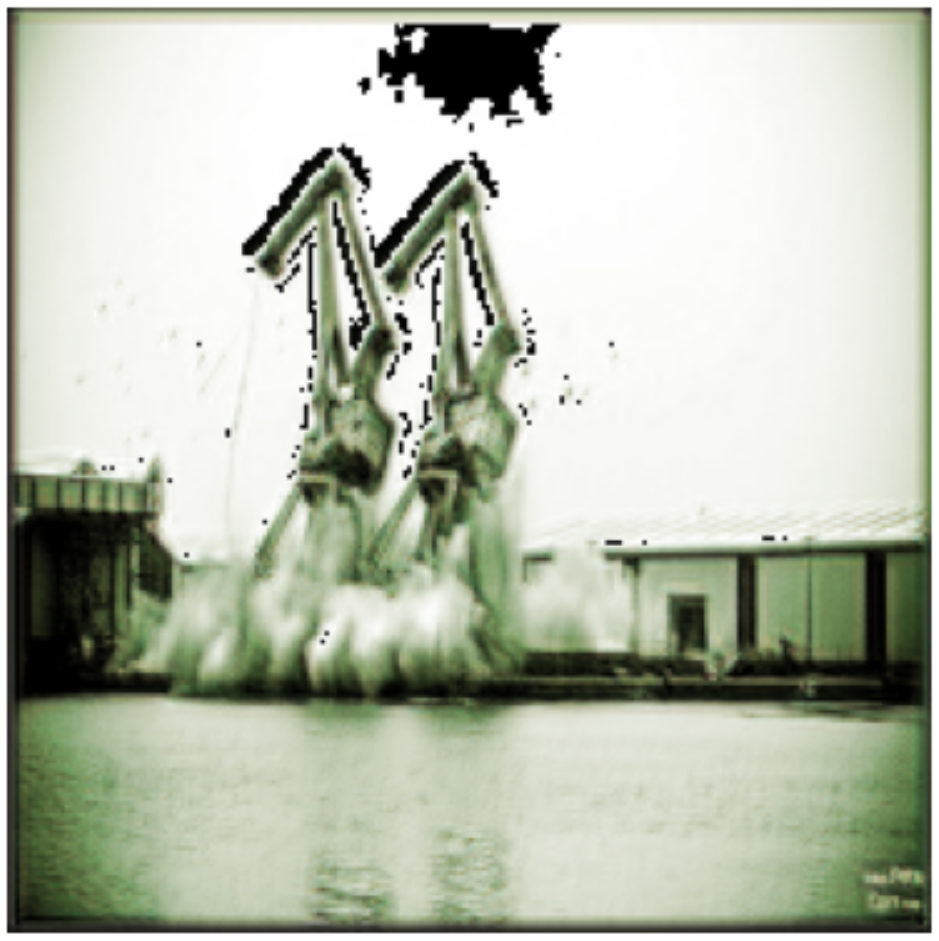
\includegraphics[scale=0.35]{m3_3.png}
		\caption{model3 colorizations}
	\end{figure}
	
	\section{Conclusions}
	While switching the colorization to HSL worked in removing the brown tint from the colorization, all the colorizations are now of a decidedly greenish tint, and many of them have artifacts, which are especially visible and egregious on results of model1 and model2. An increase in stride value has also led to a degradation of the quality of the image, so we do not intend to deviate from stride equal to 1 in the future, as the benefit from a faster convolution process are outweighed by the reduction in quality and accuracy. Filter number could be changed in the future, if more tests on filter size are conducted.
	
	\section{Plans for Future Weeks}
	In the future weeks we will continue to improve our CNN model, test more hyperparameters, and evaluate its results against other pre-trained colorizers.
	
	\section{Repository Link}
	\href{https://github.com/Daru1914/B-W-Colorising-Models}{\emph{https://github.com/Daru1914/B-W-Colorising-Models}}
	
\end{document}



